\chapter{Metodologia}
\label{cap:descr}

Seguindo o escopo abordado no capítulo anterior, uma metodologia de controlador para um bípede humanoide foi implementada. Utilizando conceitos de física e heurísticas para definir parâmetros de forma determinística, com o objetivo de gerar um padrão de caminhada ajustável e estável. Para uma melhor organização e modularidade do sistema, o controlador do bípede humanoide pode ser dividido em dois componentes com objetivos distintos: um controlador de alto nível e um controlador de baixo nível. Esta separação permite uma gestão mais eficaz das diversas tarefas e abstrações envolvidas no controle do robô.

\begin{figure}[H]
  \centering
  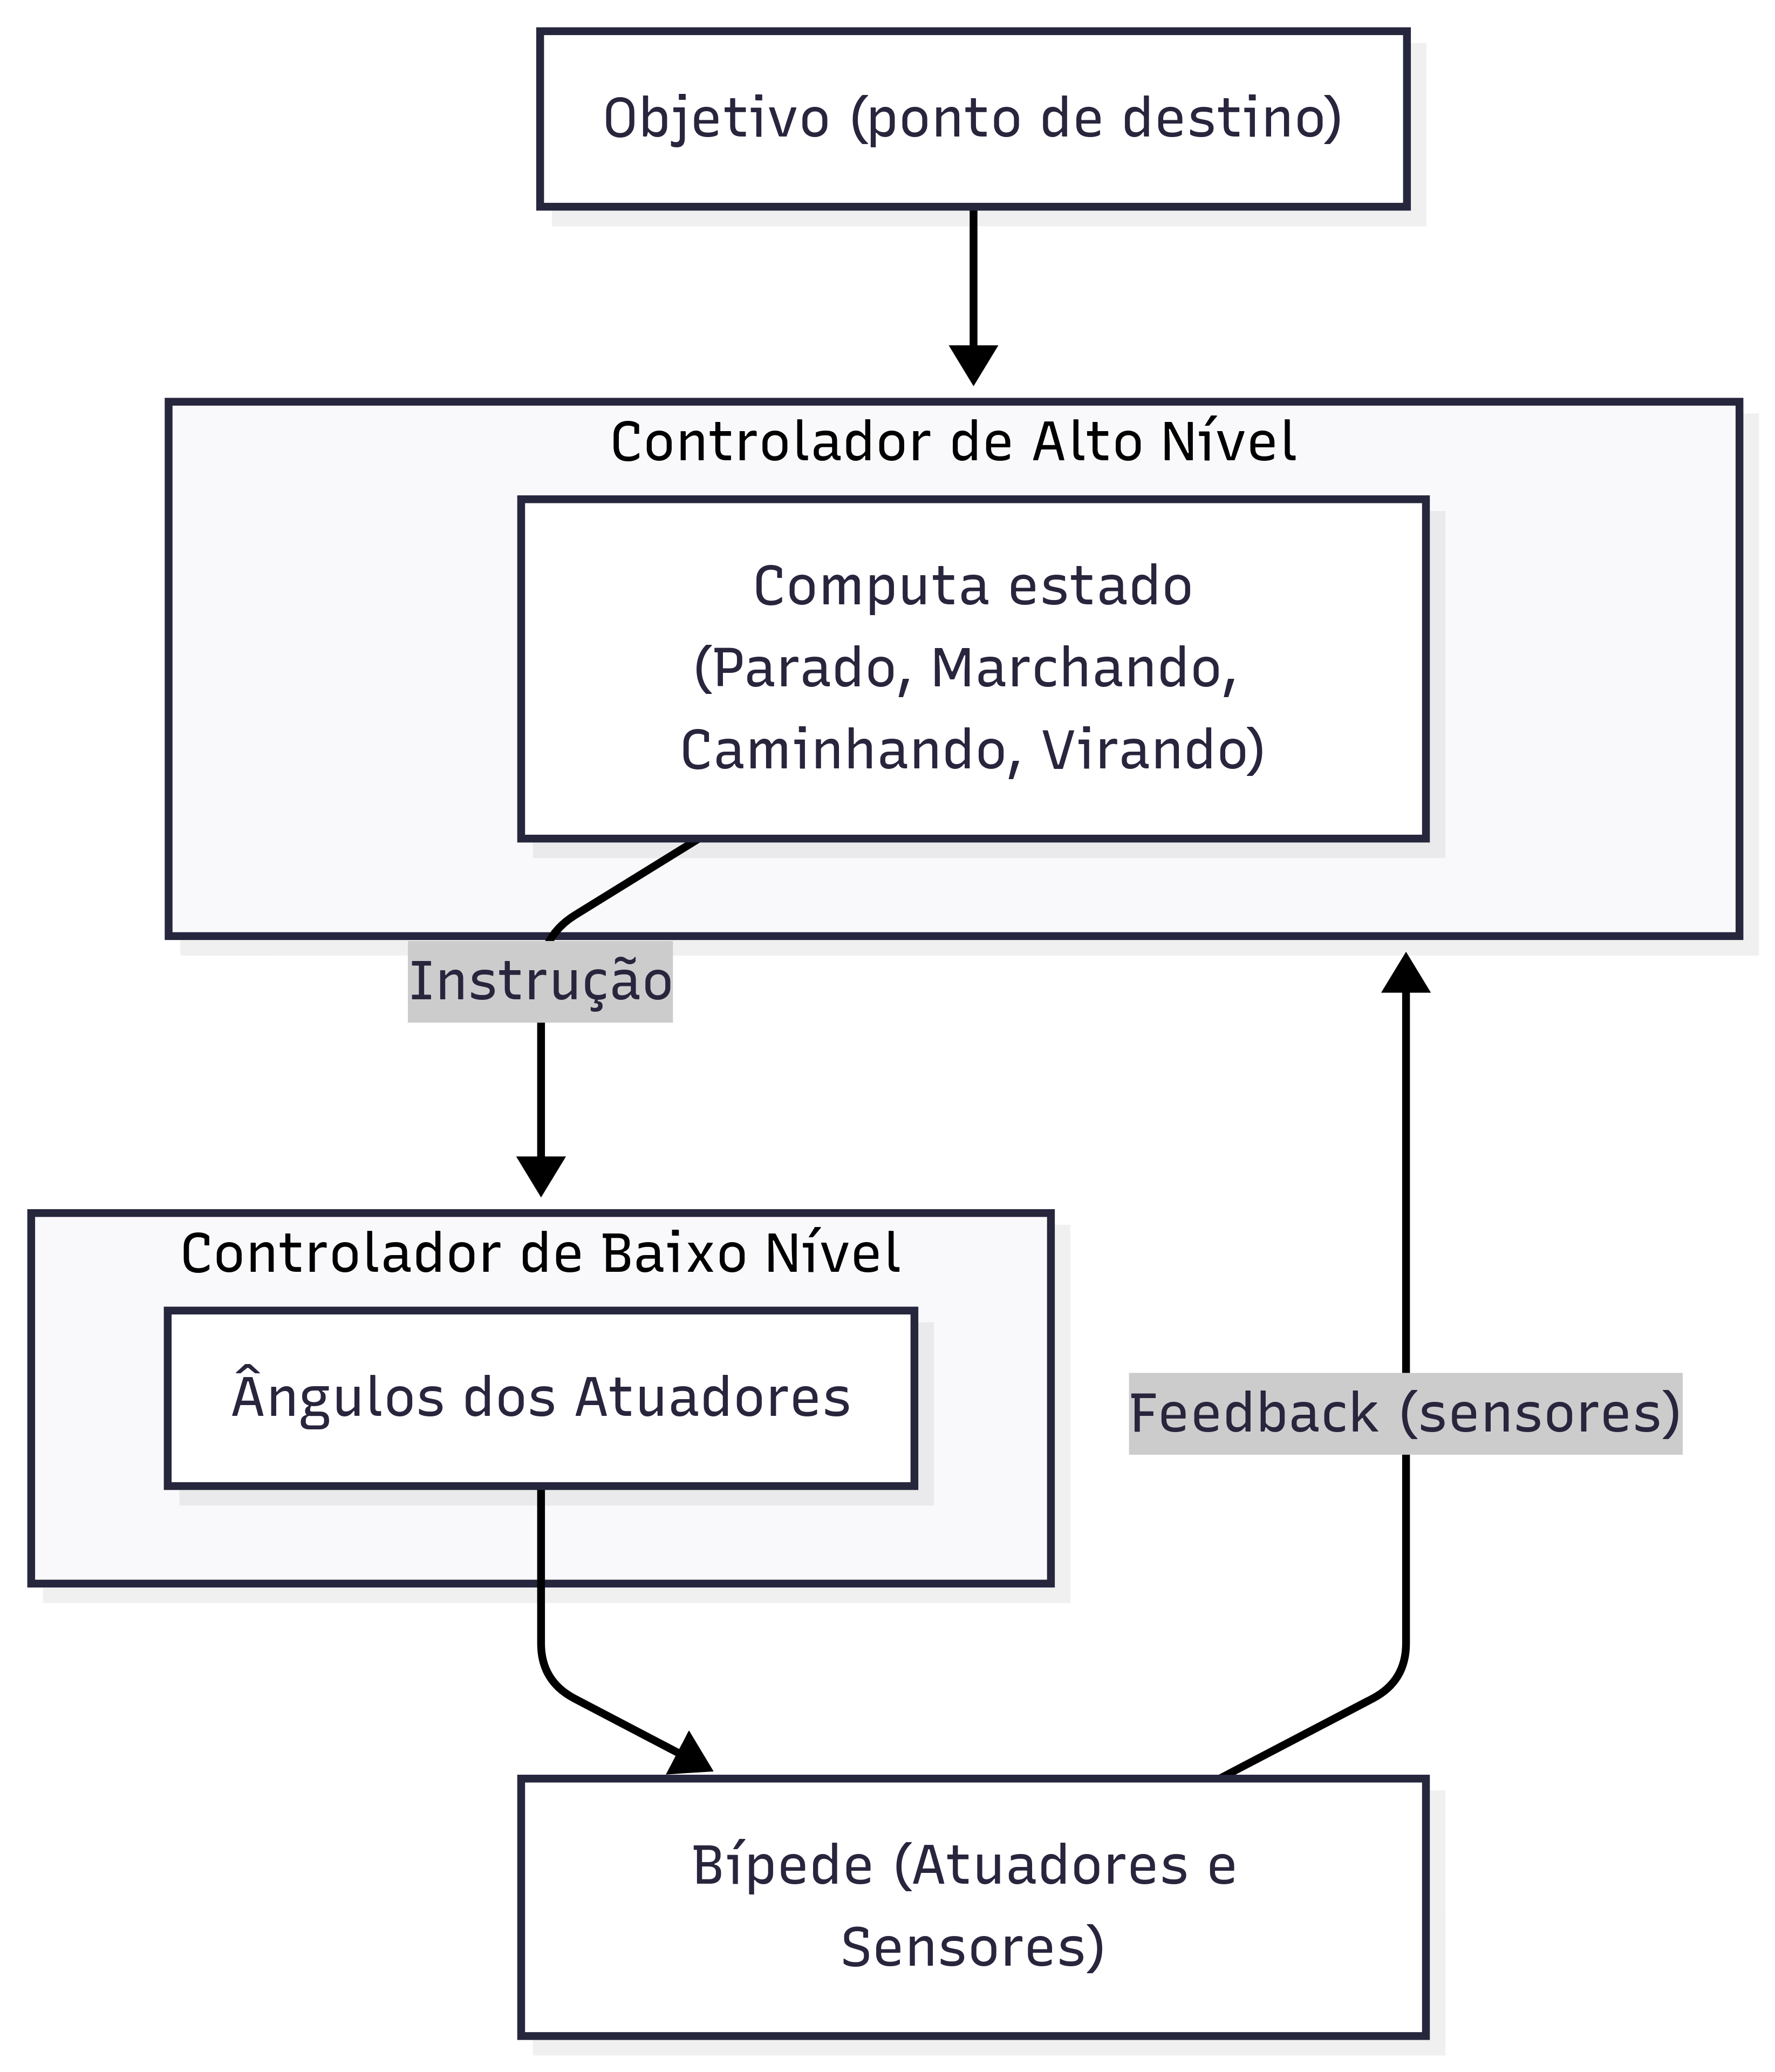
\includegraphics[width=0.7\textwidth]{./fig/fig1}
  \caption{Interação entre os controladores de alto e baixo nível, incluindo suas responsabilidades.}
  \label{fig:ctrl_niveis}
\end{figure}

O controlador de alto nível atua como o "cérebro" do sistema, tomando decisões estratégicas sobre o comportamento geral do robô. Sua responsabilidade é determinar se o robô deve andar para frente, virar à esquerda ou à direita, marchar, ou permanecer parado. Em resumo, o controlador de alto nível lida com a lógica de mais alto nível do comportamento do robô, coordenando suas ações em um nível mais abstrato.

Já o controlador de baixo nível é responsável pela execução precisa das ações definidas pelo controlador de alto nível. Suas responsabilidades incluem:
\begin{itemize}
    \item \textbf{Cinemática do bípede}: Calcular a cinemática inversa do robô, ou seja, determinar os ângulos exatos que as juntas do bípede devem ter para alcançar uma determinada pose ou orientação.
    \item \textbf{Compensar falhas mecânicas}: Aplicar métodos para compensar falhas mecânicas aumentando estabilidade do bípede durante a marcha.
\end{itemize}
O controlador de baixo nível atua como a interface direta entre o "cérebro" do bípede (controlador de alto nível) e o "corpo" do bípede (atuadores e sensores), garantindo que os comandos sejam executados gerando o movimento esperado.

\section{Controlador de Baixo Nível}
\label{sec:controlador_baixo_nivel}

O controlador de baixo nível pode ser resumido como uma equação matemática em função do tempo, que possui parâmetros que combinados produzem a ação esperada pelo controlador de alto nível. Para melhor descrever essas equações, vamos assumir que o bípede se encontra no estado "Caminhando". Assumimos também que o bípede é composto por dois manipuladores (ou conjunto de links), um representando a perna de apoio, considerando o eixo do pé como base e o eixo do quadril como extremidade, e outro representando a perna de balanço, tendo o eixo do quadril como base e o eixo do pé como extremidade. O cálculo de cinemática inversa é o cálculo dos ângulos que devem ser aplicados nos atuadores para mover suas extremidades para um determinado ponto. O controlador de baixo nível foi dividido em quatro subcomponentes:
\begin{itemize}
    \item \textbf{Gerador de pose}: Tem como objetivo gerar os pontos das extremidades dos manipuladores, representados por $p_H$ e $p_F$, sendo estas as posições do quadril da perna de apoio e a posição do tornozelo da perna de balanço respectivamente.
    \item \textbf{Gerador de cinemática}: Dados os pontos $p_H$ e $p_F$, o gerador de cinemática é responsável por calcular os ângulos que serão aplicados nos atuadores.
    \item \textbf{Função de rotação}: Tem o objetivo de gerar os ângulos dos atuadores responsáveis pela rotação do bípede.
    \item \textbf{Compensação de torque}: Este componente tem o objetivo de compensar irregularidades mecânicas causadas pela atuação da gravidade sobre as partes do bípede, gerando deltas angulares proporcionais ao torque exercido nos atuadores que exigirão mais esforço.
\end{itemize}

\subsection{Gerador de Cinemática}
\label{subsec:gerador_cinematica}

Para facilitar a definição das funções de cinemática e pose, vamos utilizar a divisão do ciclo de caminhada estabelecida em ~\cite{Perry2010} (Figura~\ref{fig:div_ciclo}), que consiste em dividimos um ciclo em duas etapas, cada etapa define qual perna estará em contato com o chão (perna de apoio) e qual perna estará se movendo para o próximo ponto (perna de balanço).

% {{PLACE_HOLDER_FIGURA_2}}
% Figura 2
\begin{figure}[H]
  \centering
  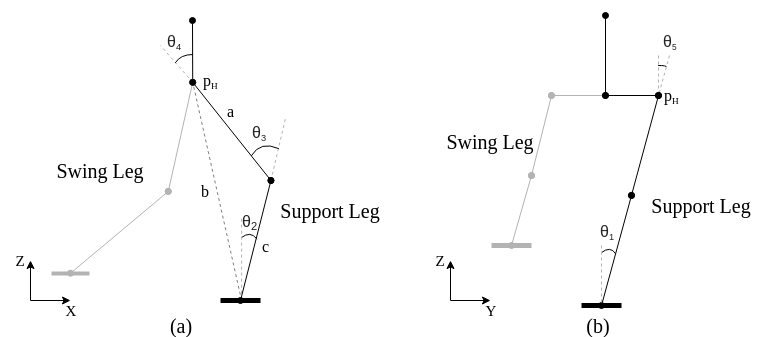
\includegraphics[width=0.7\textwidth]{./fig/fig2}
  \caption{Representação dos links da perna.}
  \label{fig:links_perna}
\end{figure}

Para calcular os ângulos dos atuadores iremos considerar que o bípede deverá estar com o tronco sempre ereto, e além disso, o quadril estará sempre rebaixado de tal forma que os dois maiores links da perna (link entre as juntas do quadril e joelho, e entre as juntas do joelho e o tornozelo) juntamente com um link imaginário entre as juntas do quadril e do tornozelo formem um triângulo, onde os lados são conhecidos ou possivelmente calculados (no caso do link imaginário). Uma vez que os lados deste triângulo são conhecidos, podemos inferir os ângulos necessários para que o bípede seja posicionado conforme o ponto $p_H$ ou $p_F$ fornecido. Considerando que o ponto informado seja $p_H$, as equações para $\theta_2$, $\theta_3$, $\theta_4$ são definidas a seguir:

\begin{equation}
    \label{eq:theta2}
    \theta_2 = \tan^{-1}(x/z) + \cos^{-1}\left(\frac{a^2-b^2-c^2}{-2bc}\right)
\end{equation}
\begin{equation}
    \label{eq:theta3}
    \theta_3 = \cos^{-1}\left(\frac{b^2-a^2-c^2}{-2ac}\right) - \pi
\end{equation}
\begin{equation}
    \label{eq:theta4}
    \theta_4 = \cos^{-1}\left(\frac{c^2-a^2-b^2}{-2ab}\right) - \tan^{-1}(x/z)
\end{equation}

Em relação ao eixo roll (eixo X), podemos observar um triângulo retângulo, onde os lados adjacentes a $\theta_1$ são conhecidos, e portanto a equação para a junta roll do tornozelo e quadril é dada por:
\begin{equation}
    \label{eq:theta1}
    \theta_1 = \tan^{-1}(y/z)
\end{equation}
\begin{equation}
    \label{eq:theta5}
    \theta_5 = -\theta_1
\end{equation}

\subsection{Gerador de pose}
\label{subsec:gerador_de_pose}

Nesta seção será descrito como usamos heurísticas e informações do modelo físico do bípede para gerar $p_H$ e $p_F$. Dado que conhecemos o padrão de caminhada humano como ilustrado na Figura~\ref{fig:div_ciclo}, podemos compor funções que se assimilam ao movimento realizado pelos pontos do pé e quadril. Estas funções têm a duração de metade do ciclo de caminhada, sendo assim, são necessárias duas delas para completar o período da marcha. Na primeira metade, a perna de apoio recebe o ponto $F_H(t)$ enquanto a perna de balanço recebe o ponto $F_F(t)$ que serão usados pelo solucionador cinemático definido anteriormente.

% {{PLACE_HOLDER_FIGURA_3}}
% Figura 3
\begin{figure}[H]
  \centering
  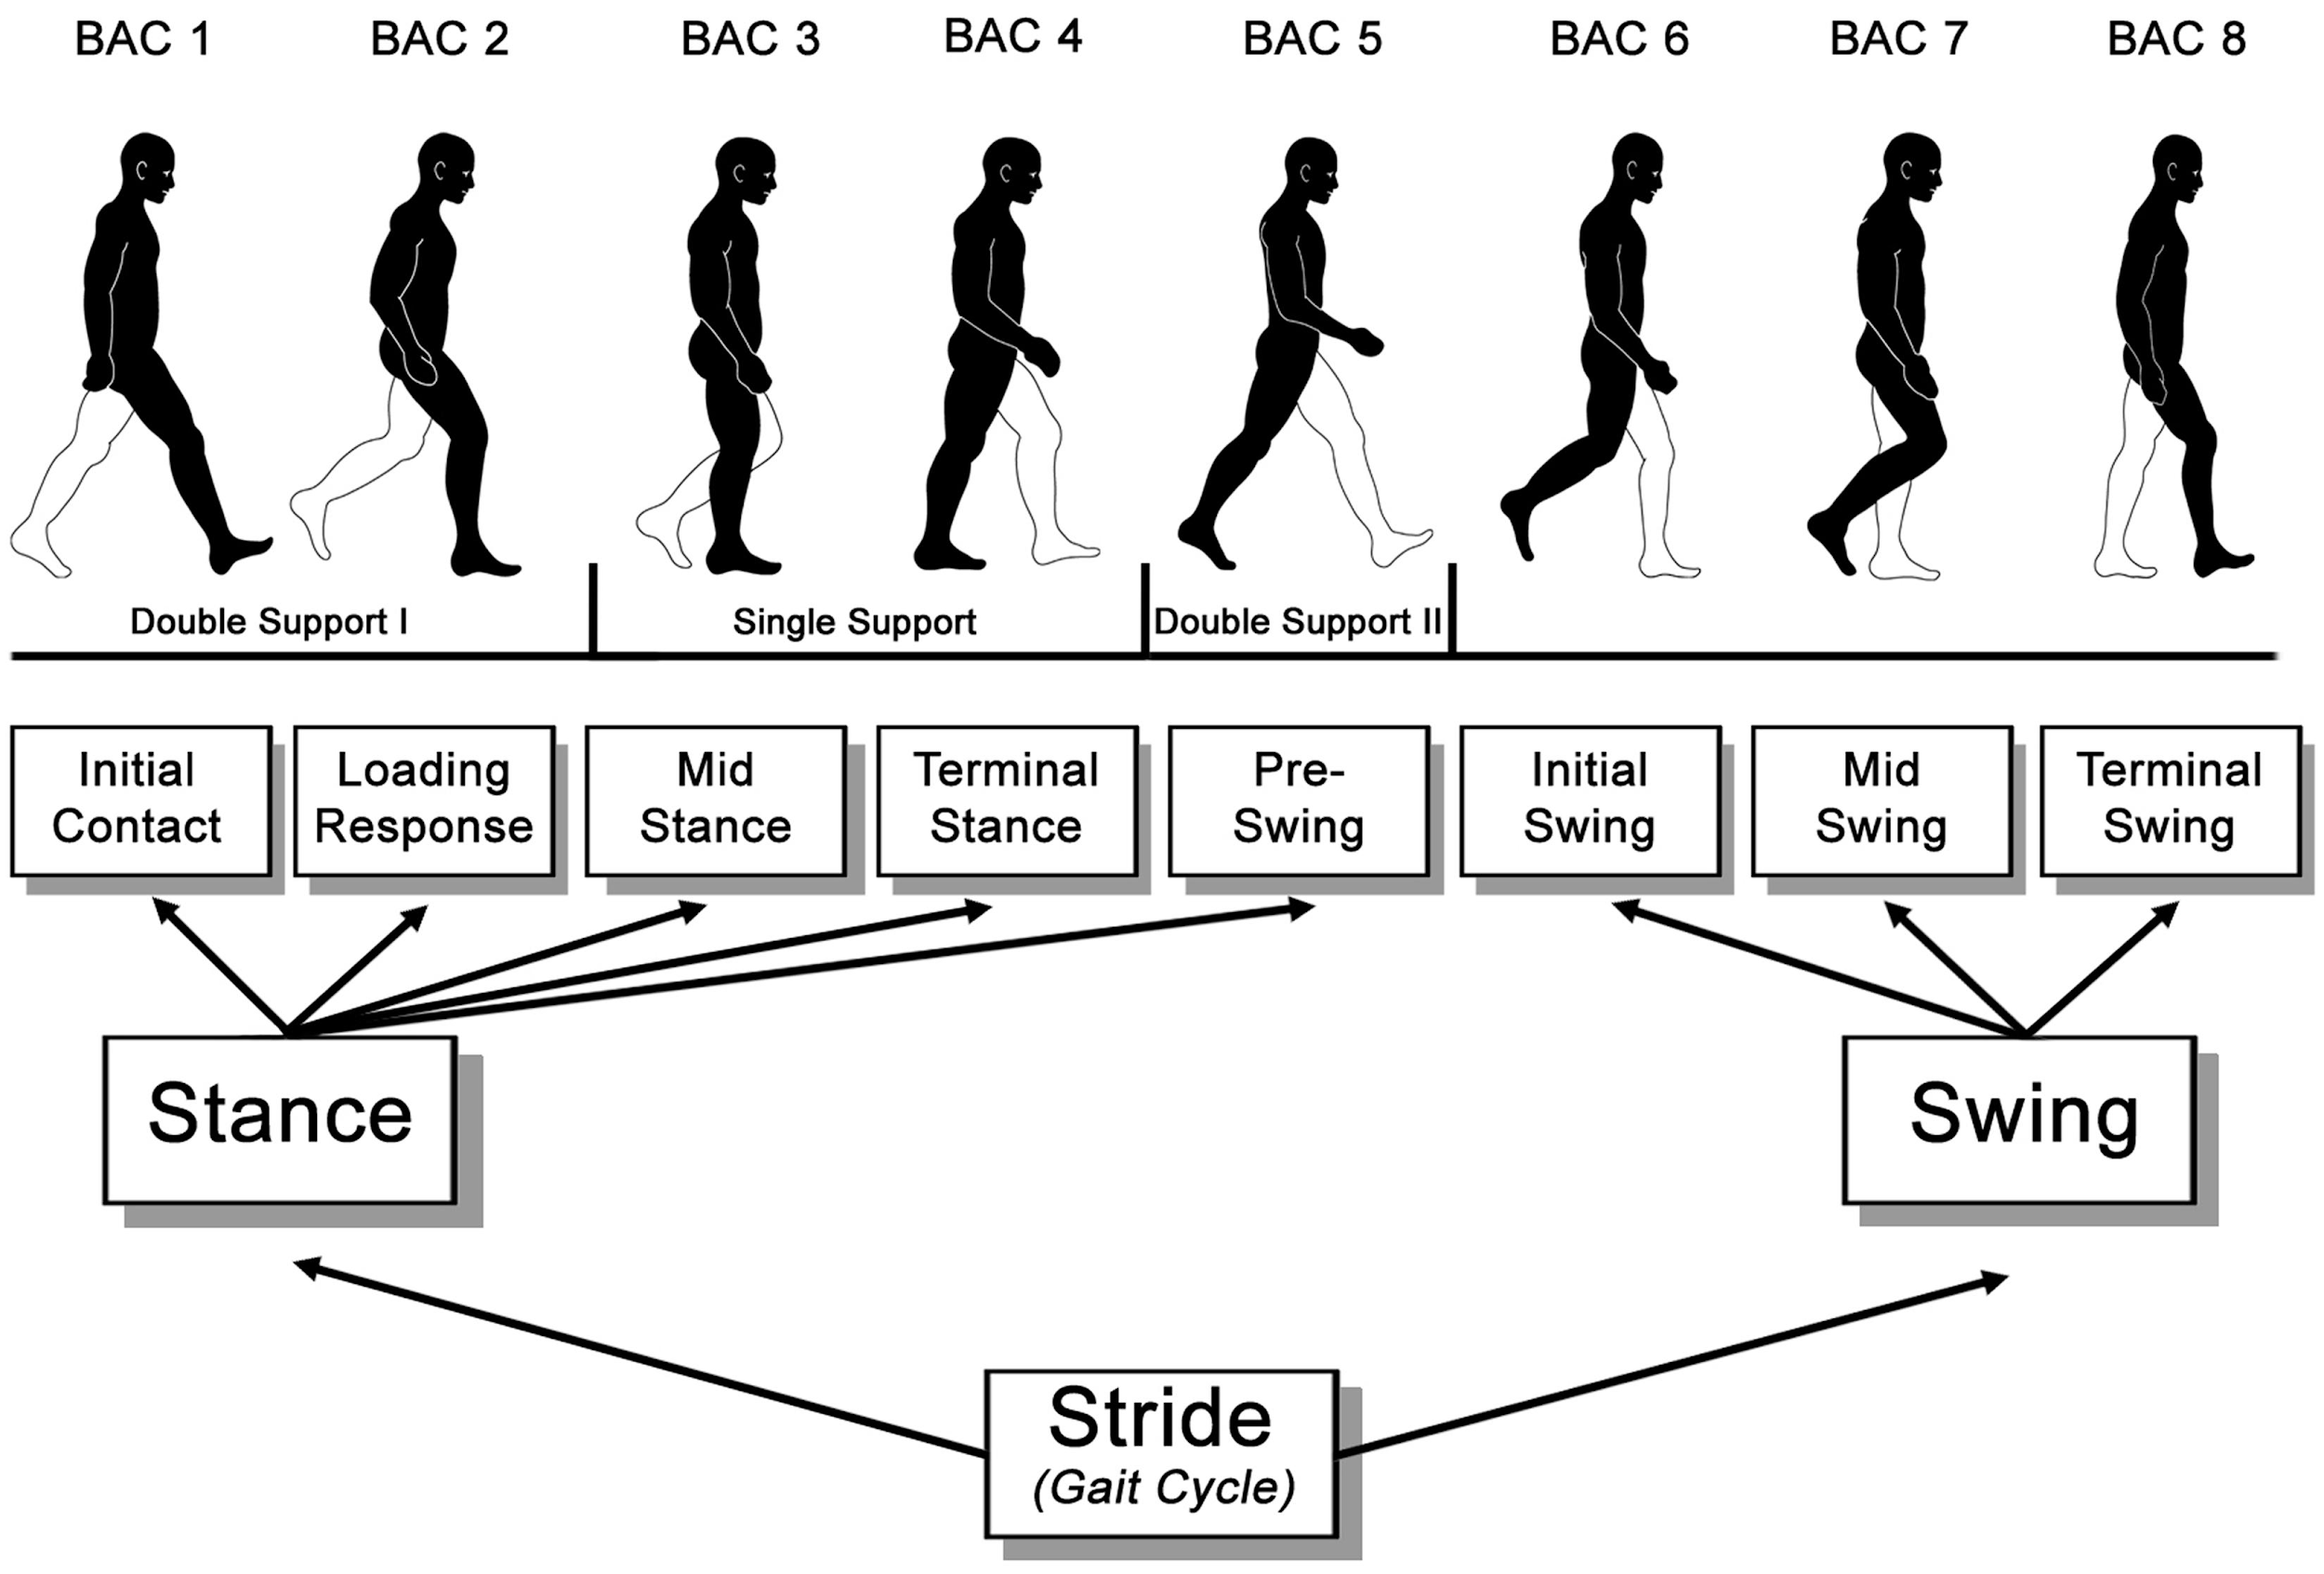
\includegraphics[width=0.7\textwidth]{./fig/fig3}
  \caption{Divisão do ciclo de caminhada segundo Perry e Burnfield~\cite{Perry2010}.}
  \label{fig:div_ciclo}
\end{figure}

\subsubsection{Função de trajetória baseada no ZMP}
\label{subsubsec:funcao_trajetoria_zmp}

Como descrito em \cite{Vukobratovic2004}, podemos dizer que o equilíbrio do bípede pode ser alcançado quando:

\begin{figure}[H]
  \centering
  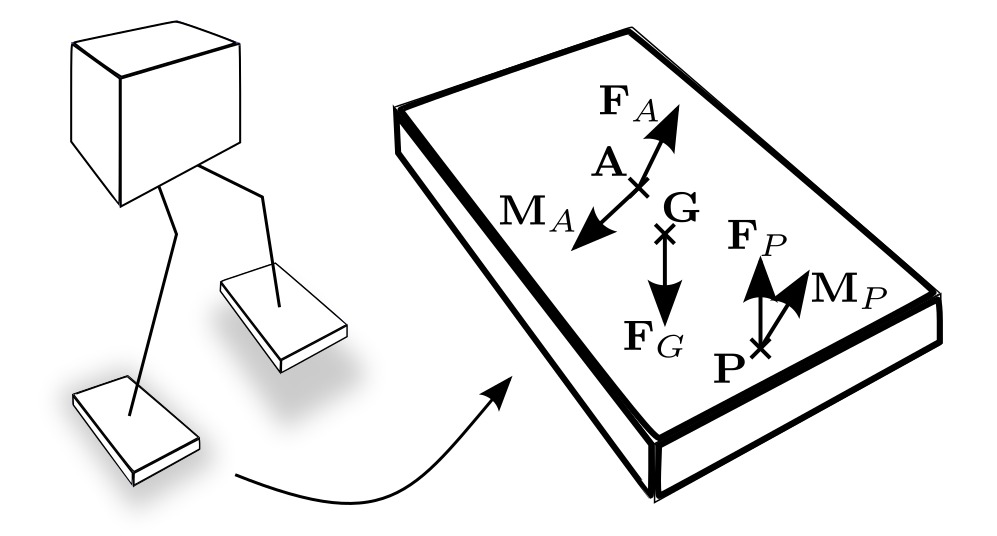
\includegraphics[width=0.7\textwidth]{./fig/fig11.jpeg}
  \caption{Forças e momentos atuando no pé de suporte durante a fase single supporte, onde apenas um pé está em contato com o chão. Imagem retirada de ~\cite{Maximo2017}}
  \label{fig:abstracao_zmp_pe}
\end{figure}

\begin{enumerate}
    \item A soma das forças $\vec{F}_A$ atuando sobre o ponto $A$ (junta do tornozelo), obtida pelo movimento conjunto das partes do corpo, e $\vec{F}_G$, provocada pela ação da gravidade no centro de massa $G$, são anuladas pela força de reação do contato com o chão $\vec{F}_P$ aplicada sobre o ponto de pressão $P$, como mostra a equação~\ref{eq:forcas_equilibrio}. Assumindo que o pé em contato com o chão não deslizará, as componentes horizontais $[F_{a,x}, F_{a,y}]$ serão anuladas pela força de fricção (componentes horizontais de $\vec{F}_P$).
    \item A soma dos momentos do corpo $\vec{M}_A$, e momento gerado por $\vec{F}_A$ são anulados pela componente vertical do momento resultante gerado pelo contato com o chão $M_{p,z}$ e pelo posicionamento horizontal de $P$ (caso $P$ esteja sobre a superfície de contato), de forma com que o braço de alavanca seja compensado por $F_{p,z}$ aplicado em $[p_x, p_y, 0]$, este ponto é denominado ZMP. Podemos dizer que uma condição necessária e suficiente para o equilíbrio dinâmico é que o momento resultante computado $\vec{M}_P$ tomando $P$ como a origem do sistema de coordenadas não produzirá componentes horizontais, ou seja $M_{p,x} = M_{p,y} = 0$. Com isso chegamos a equação~\ref{eq:momentos_equilibrio}, que é a base para o cálculo do ZMP.
\end{enumerate}

\begin{equation}
    \label{eq:forcas_equilibrio}
    \vec{F}_P + \vec{F}_G + \vec{F}_A = 0
\end{equation}

\begin{equation}
    \label{eq:momentos_equilibrio}
    \overrightarrow{OP} \times \vec{F}_P + \overrightarrow{OG} \times \vec{F}_G + \vec{M}_A + [0,0,M_{p,z}]^T + \overrightarrow{OA} \times \vec{F}_A = 0
\end{equation}

Onde $O$ é origem de um sistema de coordenadas arbitrário (geralmente o centro do pé em relação as componentes horizontais) e $\overrightarrow{OX}$ um vetor do ponto $O$ para o ponto $X$. Para satisfazer a condição 2 listada acima, o ZMP calculado precisa residir sobre a superfície de contato com o chão (SC), porém, podem haver situações em que ele precise extrapolar os limites das bordas de SC. Este comportamento resulta em tombamento, e portanto as funções $F_F(t)$ e $F_H(t)$ responsáveis por gerar a posição dos pés de balanço e quadril da perna de apoio respectivamente, devem produzir soluções que com a resolução do sistema de equações~\ref{eq:forcas_equilibrio} e~\ref{eq:momentos_equilibrio} não gere $P$ fora da SC. Além disso, a resolução da equação~\ref{eq:momentos_equilibrio} para obter a posição do CoM (Centro de Massa) a partir de um dado ZMP ou vice-versa, pode ser aproximada por modelos como o 3D-LIPM (3D Linear Inverted Pendulum Mode) introduzido em \cite{Kajita2001}, a partir da seguinte equação:

\begin{equation}
    \label{eq:3d_lipm}
    a_{CoM} - \frac{h}{g}\ddot{a}_{CoM} = a_{ZMP}
\end{equation}

Onde $a \in \{x, y\}$, h representa a altura do CoM ($z_{CoM}$), $g$ a aceleração da gravidade (9,80665 m/s²), $a_{CoM}$ e $a_{ZMP}$ sendo a posição (nos eixos x,y) do CoM e ZMP respectivamente. Dado a posição atual centro de massa ($a_{CoM}$), poderíamos calcular as posições futuras de tal forma que a aceleração final produzida ($\ddot{a}'_{CoM}$) leve a posição final do ZMP ($a'_{ZMP}$) para dentro da base definida pela SC. Para isso, precisaríamos para cada $a_{CoM, i}$ intermediário, gerar o conjunto de pontos $\{p_{H, i}$ e $p_{F, i}\}$ não distante do seu sucessor e antecessor (para que a interpolação seja possível dada a velocidade máxima das juntas). Além disso, ao invés de modificar $\ddot{a}'_{CoM}$ para obter equilíbrio, também poderíamos gerar posições futuras para os pés, fazendo com que $a'_{ZMP}$ coincida com a SC neste momento futuro. Para solucionar este problema podemos utilizar um algoritmo de otimização, onde é necessário a elaboração de uma função a ser minimizada (ou maximizada), gerando no processo um plano de caminhada satisfatório, abordagem utilizada em \cite{Maximo2017}.

\subsubsection{Função de trajetória proposta}
\label{subsubsec:funcao_trajetoria_proposta}

A partir da equação~\ref{eq:3d_lipm} podemos observar que quando a aceleração do CoM tende para 0, $a_{ZMP}$ tende para $a_{CoM}$. Isso significa que quando o bípede está parado ou se movimentando de maneira com que haja pouca aceleração do CoM, para se manter em equilíbrio, a posição do CoM (x, y) precisa residir sobre a superfície de contato. Como podemos ver no ciclo na Figura~\ref{fig:div_ciclo}, o ciclo de caminhada possui fases onde apenas um dos pés está em contato com o chão, nesse caso, o CoM precisa se mover na direção desses pontos de contato com o chão, e vamos definir $F_H(t)$ com esse objetivo (Figura~\ref{fig:trajetorias_ph_pf}). Além disso, precisamos posicionar o pé de balanço na posição futura de contato com o chão e para isso definimos $F_F(t)$.

\begin{figure}[H]
  \centering
  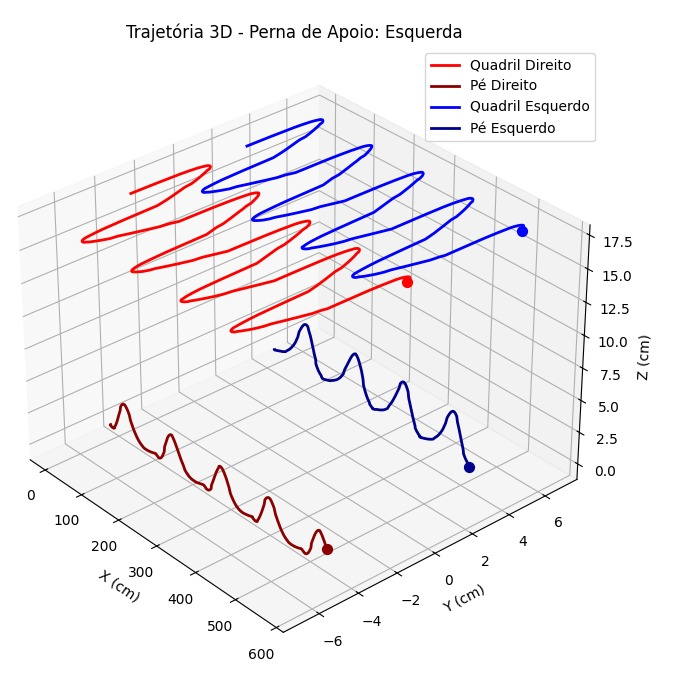
\includegraphics[width=0.7\textwidth]{./fig/trajetorias_ph_pf.jpeg}
  \caption{Trajetórias do quadril e pés durante o ciclo de caminhada. O quadril se desloca lateralmente e para frente, enquanto o pé de balanço se desloca para frente e para cima.}
  \label{fig:trajetorias_ph_pf}
\end{figure}

Começando por $F_H(t)$:

\begin{align}
    \label{eq:trajetoria_quadril}
    T_{pr}(t) &= \frac{t - T_{passo}/2}{T_{passo}/\sigma_{tanh}} \\
    F_{H,x}(t) &= p_{H}^x = \frac{d_{feet}}{2}\left(\frac{\exp(T_{pr}(t)) - \exp(-T_{pr}(t))}{\exp(T_{pr}(t)) + \exp(-T_{pr}(t))}\right) \\
    F_{H,y}(t) &= p_{H}^y = -l_{hip}\sin\left(\frac{\pi t}{T_{passo}}\right) \\
    F_{H,z}(t) &= p_{H}^z = h_{hip}
\end{align}

Onde $T_{passo}$ é o tempo de um passo e metade do ciclo de caminhada, $d_{feet}$ é a distância entre os pés na fase \textit{double support} (Figura~\ref{fig:div_ciclo}), $l_{hip}$ é o deslocamento lateral máximo do quadril e $h_{hip}$ é a altura fixa do quadril. Como podemos observar, $p_{H}^x$ é dado pela equação tanh (Tangente Hiperbólica), onde o parâmetro $\sigma_{tanh}$ será ajustado para que o bípede não tente mover o quadril para frente antes do CoM estar sobre ou próximo da SC. A componente $p_{H}^y$ representa o deslocamento lateral do quadril com amplitude $l_{hip}$, e consequentemente o de $y_{CoM}$. A função $F_F(t)$ é similar a função $F_H(t)$ em relação aos componentes horizontais, com a diferença de que $p_{F}^y$ é igual a $-p_{H}^y$ para evitar que as pernas se colidam durante a caminhada. Note que $p_{F}^x$ também segue o comportamento de uma função tanh, devido ao problema de tentar mover o pé de balanço sem que o ZMP esteja sobre o próximo pé de apoio.
A equação para o eixo z de $p_{F}$ é representada pela função sino:

\begin{equation}
    \label{eq:trajetoria_pe}
    F_{F,z}(t) = p_{F}^z = u_{foot}\exp\left(-\frac{(t-T_{passo}/2)^2}{(\sigma_{sino}T_{passo}/2)^2}\right)
\end{equation}

Onde $u_{foot}$ é a altura máxima que o pé de balanço alcançará durante o passo e $\sigma_{sino}$ um parâmetro que é ajustado manualmente para que o bípede não tente tirar o pé do chão nos momentos iniciais do passo.

\subsection{Função de Rotação}
\label{subsec:funcao_rotacao}

A rotação do bípede é realizada através da aplicação de ângulos no eixo yaw do quadril. Para controlar a direção da rotação, definimos uma variável $RT$: $RT=-1$ indica uma rotação para a esquerda, e $RT=1$ indica uma rotação para a direita. Os ângulos são calculados utilizando duas funções baseadas na tangente hiperbólica: $\tanh_{[0-1]}(t)$, que varia de 0 a 1, e $\tanh_{[1-0]}(t)$, que varia de 1 a 0.

As funções são definidas como:

\begin{align}
    \label{eq:tanh_01}
    \tanh_{[0-1]}(t) &= \frac{1 + \frac{\exp(T_{pr}(t)) - \exp(-T_{pr}(t))}{\exp(T_{pr}(t)) + \exp(-T_{pr}(t))}}{2} \\
    \label{eq:tanh_10}
    \tanh_{[1-0]}(t) &= \frac{1 - \frac{\exp(T_{pr}(t)) - \exp(-T_{pr}(t))}{\exp(T_{pr}(t)) + \exp(-T_{pr}(t))}}{2}
\end{align}

\begin{equation}
    \label{eq:theta_yaw}
    \theta_{yaw} = \theta_{Maxyaw} \cdot RT \cdot (\tanh_{[0-1]}(t) \text{ ou } \tanh_{[1-0]}(t))
\end{equation}

Onde $\theta_{Maxyaw}$ representa o ângulo máximo que $\theta_{yaw}$ pode atingir. Este ângulo $\theta_{yaw}$ é aplicado no atuador do quadril da perna oposta à direção desejada da rotação. Assim, para rotacionar para a esquerda, aplica-se $\theta_{yaw}$ na perna direita, e vice-versa. A perna na qual o ângulo é aplicado é referida como a "\textit{perna de rotação}".

Um ciclo completo de rotação será realizada em dois passos. No primeiro passo, a \textit{perna de rotação} está em contato com o chão (perna de apoio), e a função $\tanh_{[0-1]}(t)$ é utilizada para aumentar gradualmente o ângulo do quadril. No segundo passo, a \textit{perna de rotação} torna-se a perna de balanço, e a função $\tanh_{[1-0]}(t)$ é utilizada para diminuir gradualmente o ângulo do quadril de volta a 0 (estado inicial). Este processo faz com que o bípede gire enquanto a \textit{perna de rotação} está apoiada no chão e, em seguida, corrige a postura quando esta perna é levantada.

\subsection{Compensação de torque}
\label{subsec:compensacao_torque}

A atuação da aceleração da gravidade sobre as múltiplas partes do corpo provoca torques variados sobre as juntas do bípede, além disso, a presença de falha mecânica como a folga da caixa de engrenagem também pode inviabilizar que a ação gerada resulte no estado esperado. Obtendo o torque gerado pela atuação da gravidade, podemos inferir um ângulo de correção proporcional nas juntas mais afetadas por estes fenômenos.

\begin{figure}[H]
  \centering
  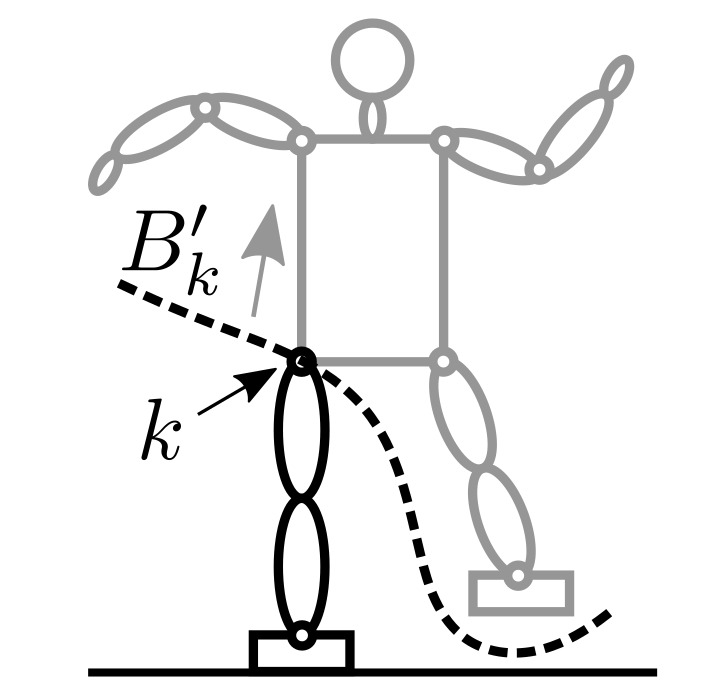
\includegraphics[width=0.7\textwidth]{./fig/compensacao_por_torque.jpeg}
  \caption{Compensação por torque em relação a junta $k$. Onde $B'_k$ é o conjunto das partes do corpo apoiadas pela junta $k$. Imagem retirada de ~\cite{Maximo2017}}
  \label{fig:compensasao_por_torque}
\end{figure}

Conforme em \cite{Maximo2017}, para cada junta $j$ onde queremos aplicar o ângulo de correção, devemos primeiro calcular $m'_j$ e $r'_{CoM, j}$, a massa total e CoM das partes apoiada por ela respectivamente:

\begin{align}
    \label{eq:mass_total}
    m'_j &= \sum_{i \in B'_j} m_i \\
    \label{eq:com_total}
    r'_{CoM, j} &= \frac{\sum_{i \in B'_j} r_{CoM, i} m_i}{m'_j}
\end{align}

Onde $B'_j$ é o conjunto das partes do corpo apoiadas por $j$. Com estas informações estamos aptos a calcular o torque exercido pela ação da gravidade em relação ao ponto da junta $j$:

\begin{equation}
    \label{eq:torque_gravidade}
    \tau'_j = r'_{CoM, j} \times [0,0,m'_j g]^T
\end{equation}

Agora precisamos obter de $\tau'_j$ a componente na direção do eixo de $j$:

\begin{equation}
    \label{eq:torque_eixo}
    \tau_{j, g} = -\tau'_j \cdot \hat{e}_j
\end{equation}

Onde $\hat{e}_j$ representa o vetor unitário que aponta em direção ao eixo de $j$. O ângulo de correção a ser aplicado em $j$ é dado por:

\begin{equation}
    \label{eq:correcao_angulo}
    \Delta\theta_{j, g} = \frac{\tau_{j, g}}{K_p}
\end{equation}

Onde $K_p$ é um parâmetro proporcional à falha mecânica (como a folga da caixa de engrenagem) apresentada pelo servo motor, este parâmetro pode ser ajustado a fim de compensar este tipo de erro de forma individual (valores especificos para cada atuador). Aplicamos este ângulo de correção apenas nas juntas do tornozelo (eixo Y, pitch) e quadril (eixo X, roll) da perna de apoio, devido ao maior esforço exigido.

\section{Controlador de Alto Nível}
\label{sec:controlador_alto_nivel}

O controlador de alto nível é responsável por determinar as ações necessárias para fazer com que o bípede cumpra seu objetivo. Ele é uma máquina de estados (Figura~\ref{fig:maq_estados}) que a cada frame computa os estados futuros do bípede com base no estado atual e objetivo geral. O objetivo geral é chegar em um determinado ponto (posição) e para isso serão calculados $d_{target}$ e $\Delta\theta_{target}$, sendo eles a distância do alvo e diferença angular necessária para rotacionar o bípede na direção do alvo respectivamente. Os estados da máquina são "Parado", "Marchando", "Caminhando" e "Virando", e podem ser descritos pela composição das variáveis $d_{feet}$, $l_{hip}$, $u_{foot}$ e $RT$, utilizadas na função de pose e rotação do bípede. A seguir vemos cada estado detalhadamente:
\begin{itemize}
    \item \textbf{Parado}: Este é o estado mais simples e é atingido quando todas as variáveis $d_{feet}$, $l_{hip}$, $u_{foot}$ e $RT$ têm valor 0.
    \item \textbf{Marchando}: A marcha é o estado onde o bípede está deslocando lateralmente o centro de massa entre as superfícies de contato com o chão e o pé de balanço está se movimentando em relação ao eixo $z$ (para cima), mas imóvel em relação ao eixo $x$ (para frente). Este estado pode ser considerado intermediário entre os demais, e pode ser alcançado quando $d_{feet}$ e $RT$ forem iguais a 0, $l_{hip}$ e $u_{foot}$ estiverem com seu valor máximo.
    \item \textbf{Caminhando}: Este é o estado onde o bípede estará caminhando para frente e é atingido quando $d_{feet}$, $l_{hip}$ e $u_{foot}$ estiverem em seu valor máximo. Neste estado não aplicamos rotação ao bípede e portanto $RT$ será igual a 0.
    \item \textbf{Virando}: Este estado é similar ao "Marchando" com a diferença que $RT$ vai possuir um valor diferente de 0, sendo -1 para virar à esquerda e 1 para a direita.
\end{itemize}

% {{PLACE_HOLDER_FIGURA_4}}
% Figura 4
\begin{figure}[H]
  \centering
  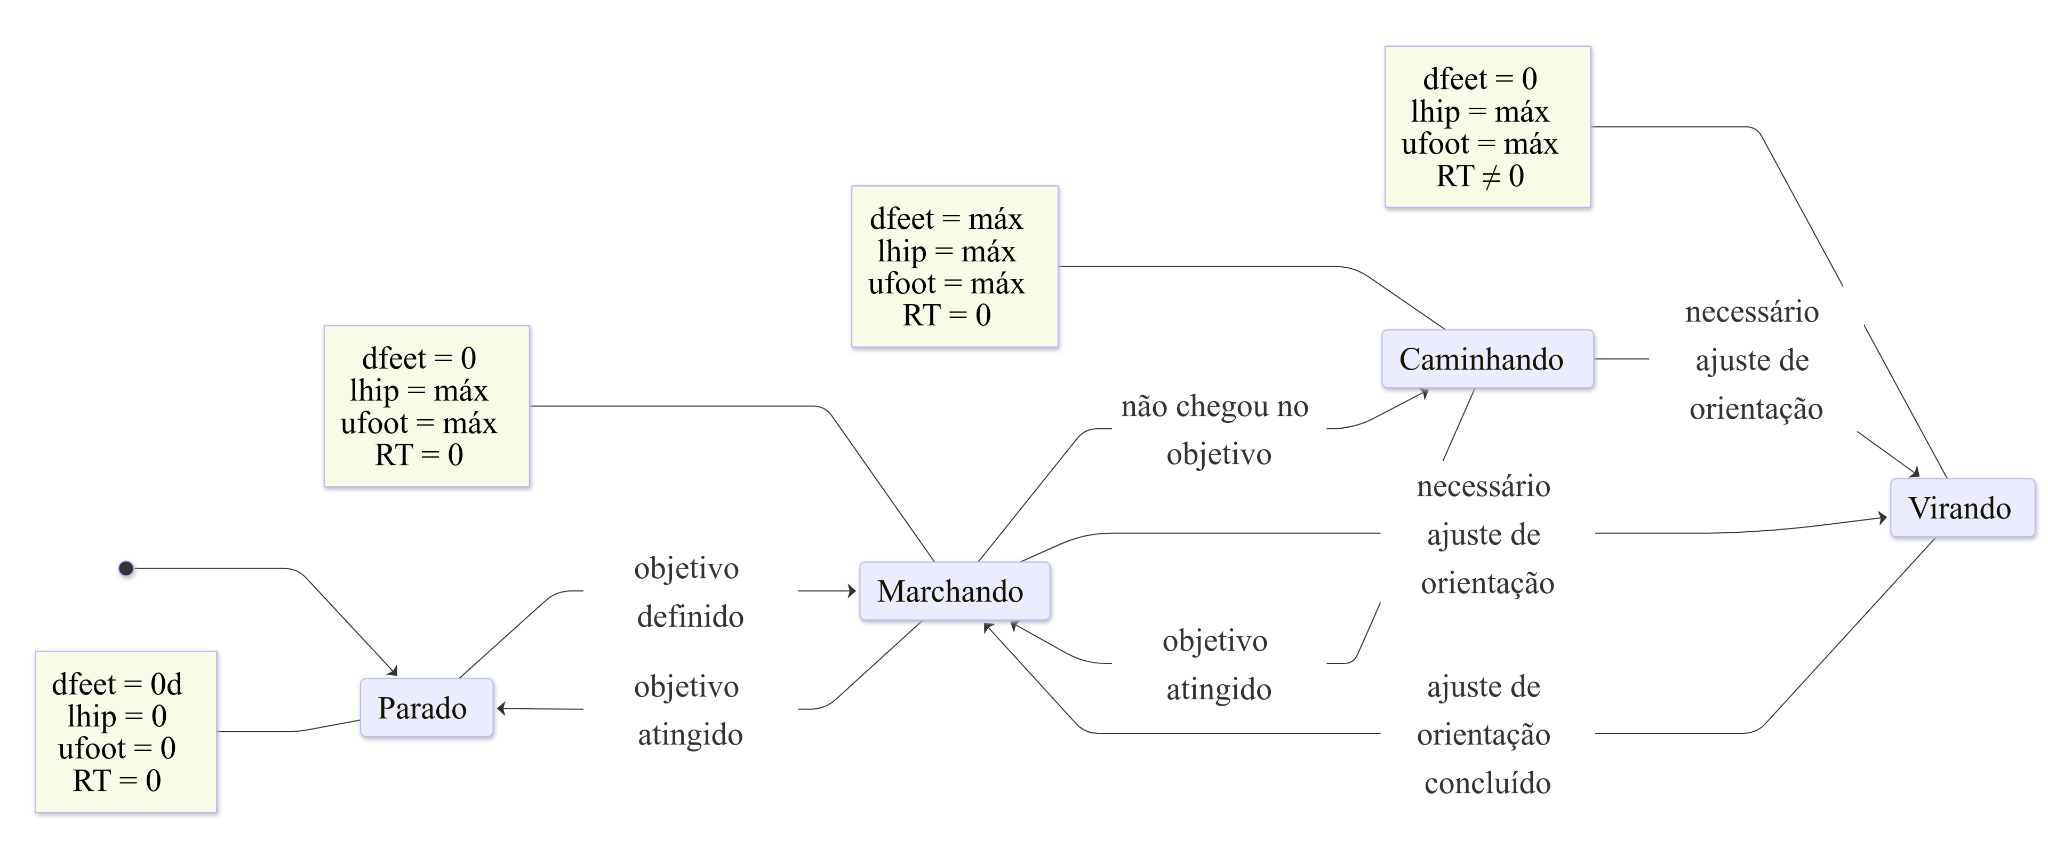
\includegraphics[width=0.7\textwidth]{./fig/fig4}
  \caption{Máquina de estados implementada pelo controlador de alto nível. As transições são definidas com base na avaliação dos parâmetros $d_{target}$ e $\Delta\theta_{target}$.}
  \label{fig:maq_estados}
\end{figure}

As transições entre os estados ocorrem por meio da interpolação linear dos valores das variáveis $d_{feet}$, $l_{hip}$ e $u_{foot}$. Os critérios para essas transições são os seguintes:
\begin{itemize}
    \item \textbf{Objetivo definido}: Um objetivo é definido quando um ponto é estabelecido como destino para o bípede.
    \item \textbf{Objetivo atingido}: O objetivo é considerado atingido quando a distância até ele $d_{target}$ é inferior a um certo limite predefinido, indicando proximidade.
    \item \textbf{Necessário ajuste de orientação}: Um ajuste de orientação é necessário quando o valor absoluto da diferença angular para o alvo ($\Delta\theta_{target}$) excede um determinado limite, sinalizando que o bípede precisa rotacionar em direção ao objetivo.
    \item \textbf{Não chegou ao objetivo}: Esta condição ocorre quando não há necessidade de ajuste de rotação ($\Delta\theta_{target}$ dentro do limite) e a distância até o objetivo ($d_{target}$) ainda é maior que o limite de proximidade.
    \item \textbf{Ajuste de orientação concluído}: O ajuste de orientação é concluído quando o valor absoluto de $\Delta\theta_{target}$ se torna menor que o limite estabelecido, indicando que o bípede está agora orientado na direção do objetivo.
\end{itemize}
